\chapter{ISPs as adversaries}\label{sec:attack_isp}

Of great importance to our approach, is aquiring real-time network traffic,
with downstream throughput being our only focus; here discuss the potential
scenarios that allow adversaries to obtain such information, and describe how,
in particular ISPs, could make use of it, to identify video streaming and
profile users based on their streaming habits.

\section{Attack Scenarios}\label{attack_scenarios}

Given the nature of modern Internet infrastructure, an adversary interested in
eavesdropping a particular communication, only needs to compromise a node on
the path the communication travels through. An \emph{on-path} attacker could
easily gain passive access to network and transport layers, and start capturing
network traffic. This can include malicious or compromised Wi-Fi access
points, routers, tapped network cables and ISPs. 

Rather than just attacking physical devices, leaks of information could occur
in network connections, in which an attacker physically close to the victim,
could make use of a \emph{Wi-Fi sniffer} to estimate traffic by capturing
physical layer WLAN packets.  Information may be encrypted by 802.11, and the
sniffer may not take into account packet retransmissions at the session layer
nor multiple TCP/IP flows on the same link, potentially causing noise on the
observation. Despite so, Reed et Al. \cite{leaky_streams}, have shown that it
is still possible to estimate WAP-to-client throughput and use it to identify
the content being streamed.

In addition to the above, \emph{side-channel eavesdropping} can exploit
information about the network structure, to saturate a link between the user
and the server, and estimate fluctuations of congestion by sending probes
remotely and observing queueing delays in routers \cite{side_channel}. 

We will now present the relevant phases and tools needed for an ISP to perform
such attack.

\section{Video Fingerprinting}

Assuming that the ISP has no direct access to the CDN, title are stored in, it
needs to build a database of video traffic to match against future video stream
captures. To build such a database, the ISP needs to have access to a network
interface, control its inbound bandwidth, (to get different levels of quality
for each title), and capture incoming traffic passing through it.

In order to control the incoming bandwidth, the ISP could either limit it
directly onto a generic L4 switch (probably more stable), or decide to connect
any UNIX-like machine and throttle the throughput of its main ethernet
interface. We will consider the scenario in which the ISP limits the bandwidth
of the ethernet interface of the switch.

The value of the enforced bandwidth determines the quality (bitrate) of the
content that will be captured. This require the ISP to choose a policy on how
to throttle the bandwidth to get all different quality levels for each title.
We assume the bandwidth levels to be the one shown in \Cref{tab:bandwidths}.
These values, in our own version of the attack, have proven to reconstruct
faithfully the bitrate ladders of each title, thus we assume the ISP to use
them as reference, although in reality, our approach would work with any set
capable of spanning the space of bitrate levels.

\begin{table}[htb]
  \centering
  \begin{tabular}{|c|c|c|c|c|c|c|c|c|c|c|c|c|}
    \hline
    \multicolumn{13}{|c|}{\textbf{Bandwidth levels (Mbps)}} \\
    \hline
    0.6 & 0.8 & 1.2 & 2 & 3.5 & 4.2 & 4.8 & 5.5 & 6.5 & 7.05 & 10 & 15 & 20 \\ 
    \hline
  \end{tabular}
  \caption{Enforced bandwidth levels.}
  \label{tab:bandwidths}
\end{table}

\todo{Explain briefly how the ISP needs to capture traffic to build the database}

\section{Capturing video traffic}

This, requires the ISP to be in possess of a generic L4 switch that can mirror
traffic from a port to another one. Then any UNIX-like system that implements
\emph{libpcap} is suitable for capturing inbound traffic on the mirrored port, as
presented below in \Cref{fig:schema}.

\begin{figure}[!htb]
  \centering
  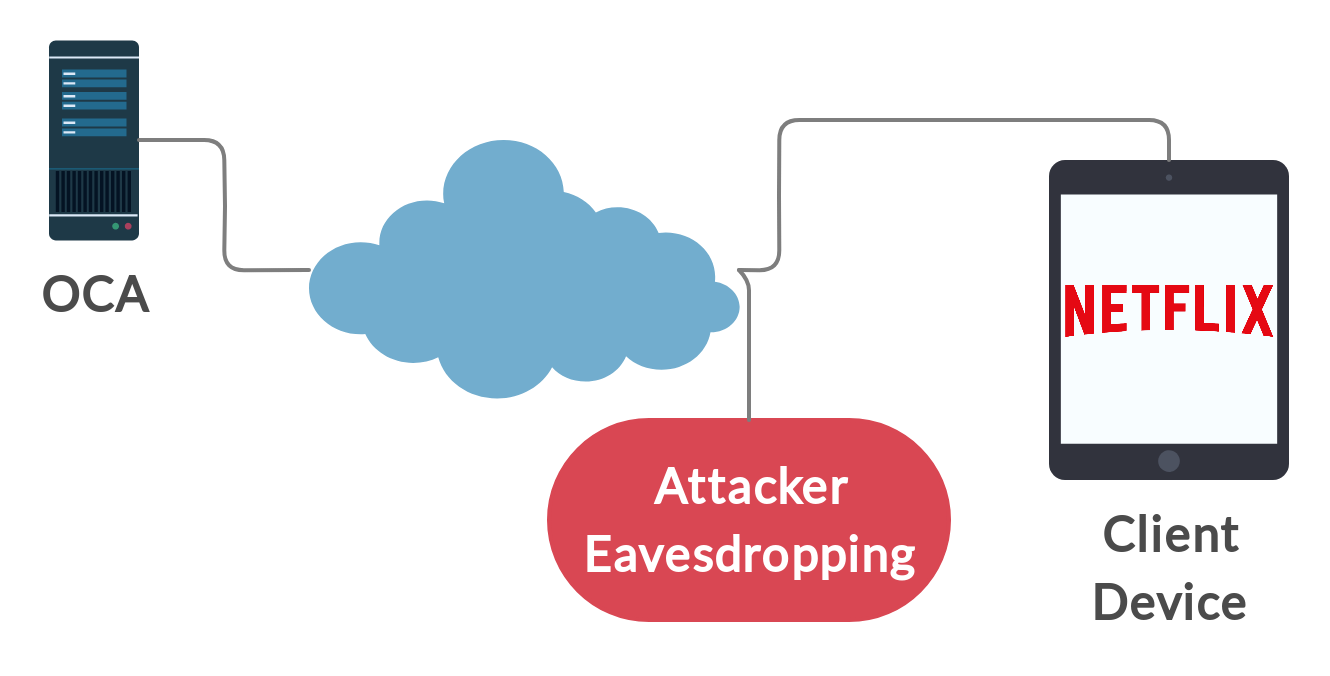
\includegraphics[width=0.9\columnwidth]{img/schema.png}
  \caption{Traffic capture scenario.}
  \label{fig:schema}
\end{figure}

The UNIX machine can now listen onto the interface to which traffic is mirrored
by invoking \texttt{tcpdump}. 
